\definecolor{zzttqq}{rgb}{0.15,0.35,0.15}

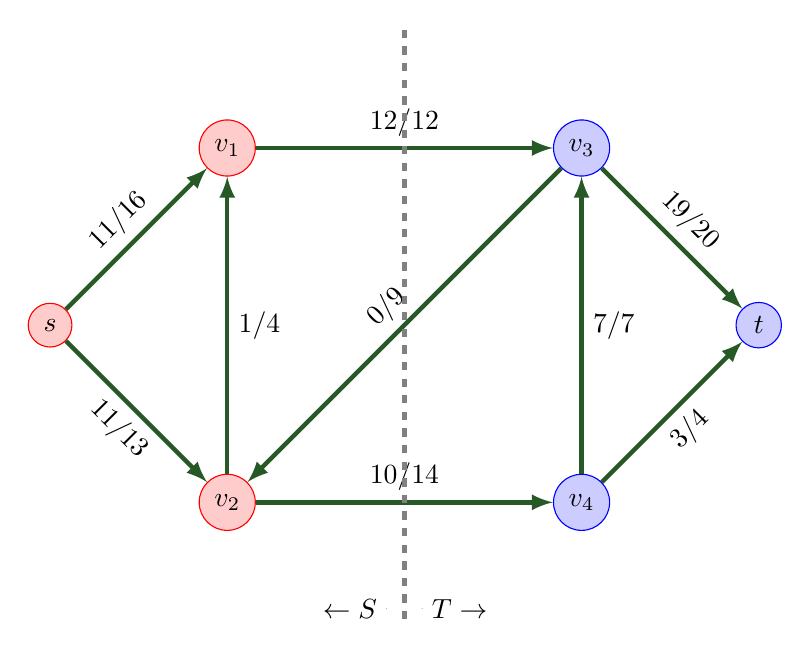
\begin{tikzpicture}[x=1.5cm, y=1.5cm]
	\fill (0.15,-2.4) circle (0.1pt)node[anchor=west] {$T\rightarrow$};
	\fill (-0.15,-2.4) circle (0.1pt)node[anchor=east] {$\leftarrow S$};
	\node[circle,draw=red,fill=red!20] (s) at (-3,0) {$s$};
    \node[circle,draw=red,fill=red!20!] (v1) at (-1.5,1.5) {$v_1$};
    \node[circle,draw=red,fill=red!20!] (v2) at (-1.5,-1.5) {$v_2$};
    
    \node[circle,draw=blue,fill=blue!20!] (v3) at (1.5,1.5) {$v_3$};
    \node[circle,draw=blue,fill=blue!20!] (v4) at (1.5,-1.5) {$v_4$};
    \node[circle,draw=blue,fill=blue!20!] (t) at (3,0) {$t$};
    
    \draw[color=zzttqq, ultra thick, -latex]  (s) edge node[rotate = 45, above,color=black]{11/16} (v1);
	\draw[color=zzttqq, ultra thick, -latex]  (s) edge node[rotate = -45, below,color=black]{11/13} (v2);
	\draw[-latex, color=zzttqq, ultra thick]  (v2) edge node[right,color=black]{1/4} (v1);
	\draw[-latex, color=zzttqq, ultra thick]  (v1) edge node[above,color=black]{12/12} (v3);
	\draw[-latex, color=zzttqq, ultra thick]  (v2) edge node[above,color=black]{10/14} (v4);
	\draw[-latex, color=zzttqq, ultra thick]  (v3) edge node[rotate=45,above,color=black]{0/9} (v2);
	\draw[-latex, color=zzttqq, ultra thick]  (v4) edge node[right,color=black]{7/7} (v3);
	\draw[-latex, color=zzttqq, ultra thick]  (v3) edge node[rotate=-45,above,color=black]{19/20} (t);
	\draw[-latex, color=zzttqq, ultra thick]  (v4) edge node[rotate=45,below,color=black]{3/4} (t);
	\draw[color=gray, ultra thick, dashed]  (0, 2.5) edge (0,-2.5);
\end{tikzpicture}